\documentclass{standalone}
\usepackage{tikz}
\usetikzlibrary{arrows,shapes,matrix,trees,fit,backgrounds,shapes,calc}
% all other packages and stuff you need for the picture
%
\begin{document}
\scalebox{.5}{
  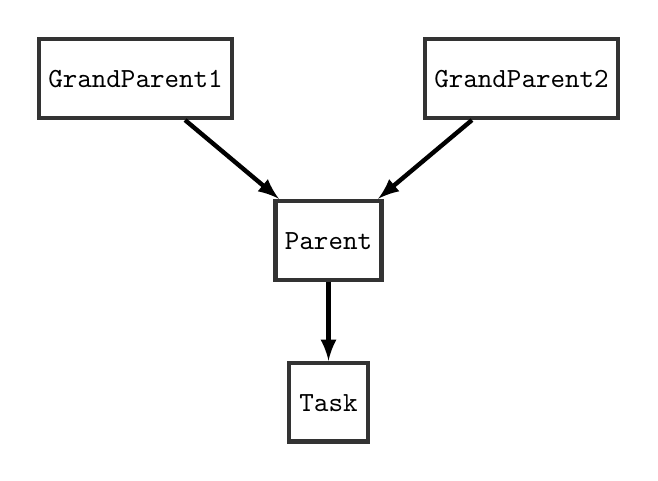
\begin{tikzpicture}[auto, ultra thick,>=latex]
    \tikzstyle{state}=[rectangle,minimum size=1cm, draw=black!80, font=\bfseries, node distance=3cm]
    \tikzstyle{every matrix} = [matrix of nodes, ampersand replacement=\&, align=right, nodes in empty cells, nodes={text height=1.5ex}, minimum width=.4cm]
    \matrix at (0,0)
    {
      \node[state] (grandparent1) {\texttt{GrandParent1}}; \&[.5cm] \&[.5cm]        \node[state] (grandparent2) {\texttt{GrandParent2}};\\[1cm]
      \& \node[state] (parent) {\texttt{Parent}}; \& \\[1cm]
      \& \node[state] (task) {\texttt{Task}}; \& \\
    };
    \draw (grandparent1) edge[->] (parent);
    \draw (grandparent2) edge[->] (parent);
    \draw (parent) edge[->] (task);
  \end{tikzpicture}
}
\end{document}

%%% Local Variables: 
%%% mode: latex
%%% TeX-master: t
%%% End: 
